\documentclass[11pt,a4paper]{article}

% -----------------------------------------------------------------------------
% Packages & Configuration
% -----------------------------------------------------------------------------
\usepackage[utf8]{inputenc}
\usepackage[margin=1in]{geometry}
\usepackage{amsmath,amssymb,amsfonts}
\usepackage{booktabs}
\usepackage{tabularx}
\usepackage{listings}
\usepackage{xcolor}
\usepackage{hyperref}
\usepackage{tikz}
\usepackage{pgfplots}
\usepackage{caption}
\usepackage{microtype}
\usepackage{enumitem}
\usepackage{fancyhdr}
\usepackage{titlesec}

\pgfplotsset{compat=1.18}
\usetikzlibrary{shapes.geometric,arrows.meta,positioning,calc}

% -----------------------------------------------------------------------------
% Color Palette & Listings Theme
% -----------------------------------------------------------------------------
\definecolor{primaryblue}{RGB}{24, 76, 120}
\definecolor{secondarygreen}{RGB}{46, 117, 89}
\definecolor{darkslate}{RGB}{38, 36, 33}
\definecolor{codegray}{RGB}{245, 245, 245}
\definecolor{commentgreen}{RGB}{34, 139, 34}
\definecolor{keywordblue}{RGB}{0, 0, 205}
\definecolor{stringred}{RGB}{178, 34, 34}

\hypersetup{
    colorlinks=true,
    linkcolor=primaryblue,
    citecolor=secondarygreen,
    urlcolor=primaryblue
}

\lstset{
    backgroundcolor=\color{codegray},
    commentstyle=\color{commentgreen}\itshape,
    keywordstyle=\color{keywordblue}\bfseries,
    stringstyle=\color{stringred},
    basicstyle=\ttfamily\footnotesize,
    breaklines=true,
    captionpos=b,
    frame=single,
    rulecolor=\color{gray!40},
    numbers=left,
    numberstyle=\tiny\color{gray},
    numbersep=6pt,
    tabsize=4,
    showstringspaces=false
}

% -----------------------------------------------------------------------------
% Header & Footer Setup
% -----------------------------------------------------------------------------
\pagestyle{fancy}
\fancyhf{}
\fancyhead[L]{\small\color{gray}Mockfish: Knowledge-Guided Adversarial Chess Engine}
\fancyhead[R]{\small\color{gray}AI with Python Coursework}
\fancyfoot[C]{\thepage}
\renewcommand{\headrulewidth}{0.4pt}
\renewcommand{\footrulewidth}{0.4pt}

% -----------------------------------------------------------------------------
% Document Title & Metadata
% -----------------------------------------------------------------------------
\title{
    \vspace{-1.5cm}
    \textbf{\Huge Mockfish: An Intelligent Knowledge-Guided Adversarial Chess Engine \& Interactive GUI} \\[0.3cm]
    \large End-Semester AI Capstone Project Report --- Artificial Intelligence with Python
}

\author{
    \textbf{Student 1} (Logic \& Rules Specialist) \quad
    \textbf{Student 2} (State Space \& Heuristics Specialist) \\
    \textbf{Student 3} (Adversarial Search Specialist) \quad
    \textbf{Student 4} (GUI \& Systems Integrator Specialist) \\[0.3cm]
    \textit{Department of Computer Science \& Engineering} \\
    \textit{University AI with Python Coursework Team} \\[0.2cm]
    \textbf{GitHub Repository}: \url{https://github.com/unclePRO/mockfish}
}
\date{\today}

% -----------------------------------------------------------------------------
% Document Content
% -----------------------------------------------------------------------------
\begin{document}

\maketitle
\thispagestyle{empty}

\begin{abstract}
This report presents the design, theoretical formulation, empirical evaluation, and full architectural implementation of \textbf{Mockfish}, an intelligent, tournament-capable adversarial chess engine and graphical user interface developed in Python. Designed to address the combinatorial explosion of discrete game trees ($\sim 10^{120}$ theoretical variations), Mockfish synthesizes multiple artificial intelligence paradigms: (1) a deterministic \textbf{Knowledge-Based Expert System} providing $O(1)$ opening book retrieval, (2) an optimized \textbf{Alpha-Beta Pruning Minimax} engine coupled with \textbf{Heuristic Move Ordering} (MVV-LVA, tactical checks, castling incentives, and promotions), (3) an advanced \textbf{State Space Evaluation} function utilizing PeSTO Piece-Square Tables (PST) and dynamic king safety metrics, and (4) an \textbf{Iterative Deepening Depth-First Search (IDDFS)} anytime formulation. Empirical benchmarks demonstrate that our heuristic move ordering achieves a \textbf{99.27\% pruning efficiency} over exhaustive Minimax, reducing the effective branching factor from $b_{eff} = 37.35$ down to $7.23$ and yielding a \textbf{156.6$\times$ computational speedup} at depth 3. The interactive Tkinter GUI resolves classical OS modal dialog freezing by implementing an in-canvas, non-blocking Game Over overlay alongside real-time search telemetry.
\end{abstract}

\vspace{0.3cm}
\tableofcontents
\newpage

% -----------------------------------------------------------------------------
% Section 1: Introduction & Real-World Application
% -----------------------------------------------------------------------------
\section{Real-World Problem Identification \& Application Domain}

\subsection{Application Domain: Autonomous Adversarial Game-Playing}
In accordance with coursework specifications, our team selected the domain of an \textbf{Intelligent Game-Playing Agent} for chess. In the historical evolution of artificial intelligence, chess has served as the foundational benchmark for exploring how machines represent knowledge, navigate vast search graphs, reason under uncertainty, and optimize sequential decisions in the presence of an active adversary.

\subsection{Real-World Significance \& Transferability}
While embodied in a two-player board game, the exact algorithmic mechanisms implemented in Mockfish directly address core challenges across modern industrial and enterprise domains:
\begin{enumerate}[leftmargin=*]
    \item \textbf{Adversarial Multi-Agent Systems}: In financial electronic trading, algorithmic agents must make rapid capital allocations while competing against rival algorithms seeking to exploit order flow. Similarly, automated cybersecurity response agents operate in zero-sum environments defending networks against persistent adversaries. Minimax and Alpha-Beta formulations provide mathematical optimality guarantees under worst-case assumptions.
    \item \textbf{High-Dimensional Combinatorial Optimization}: With an average branching factor of $b \approx 35$ and legal game configurations exceeding $10^{40}$ states, chess cannot be solved by brute force. The branch-and-bound pruning, heuristic state space reduction, and move prioritization algorithms developed here translate directly to airline crew scheduling, parcel routing, and supply chain logistics.
    \item \textbf{Hybrid Decision Architectures}: Expert systems in clinical decision-support and industrial automation combine instant knowledge-base lookups for standard, codified protocols with dynamic, compute-heavy heuristic reasoning when encountering rare, off-nominal scenarios. Mockfish mirrors this by coupling an $O(1)$ propositional opening database with a multi-ply adversarial search engine.
\end{enumerate}

% -----------------------------------------------------------------------------
% Section 2: Problem Formulation
% -----------------------------------------------------------------------------
\section{Formal Problem Formulation}

We formulate chess as a discrete, deterministic, turn-based, zero-sum, perfect-information adversarial environment formally defined by the tuple:
$$\mathcal{M} = \langle S_0, Actions, Result, Constraints, Terminal\_Test, Utility, Heuristic \rangle$$

\begin{figure}[htbp]
\centering
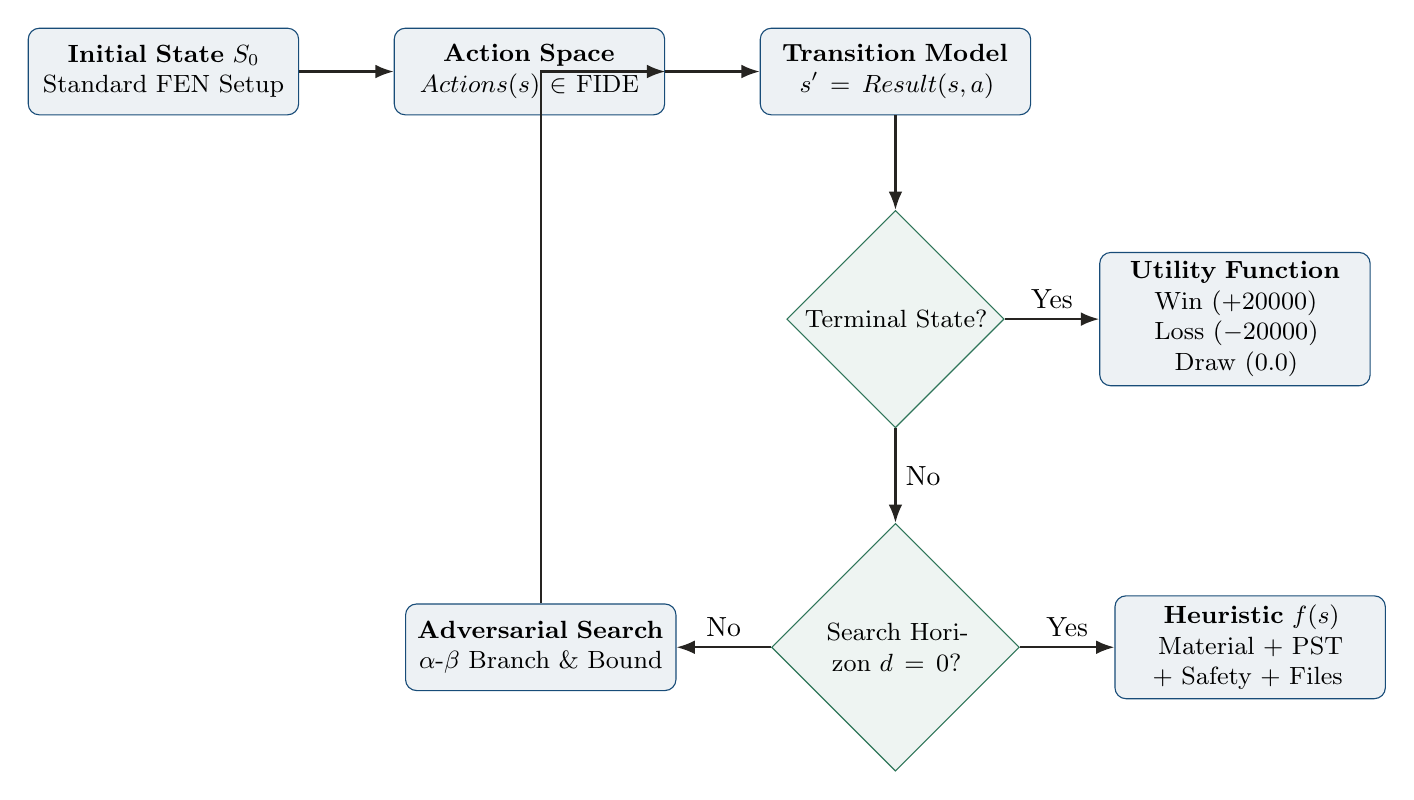
\begin{tikzpicture}[node distance=1.5cm, auto,
    block/.style={rectangle, draw=primaryblue, fill=primaryblue!8, text width=3.2cm, text centered, rounded corners, minimum height=1.1cm, font=\small},
    decision/.style={diamond, draw=secondarygreen, fill=secondarygreen!8, text width=2.4cm, text centered, inner sep=1pt, font=\small},
    line/.style={draw=darkslate, -Latex, thick}]

    \node [block] (init) {\textbf{Initial State $S_0$}\\Standard FEN Setup};
    \node [block, right=1.2cm of init] (act) {\textbf{Action Space}\\$Actions(s) \in \text{FIDE}$};
    \node [block, right=1.2cm of act] (trans) {\textbf{Transition Model}\\$s' = Result(s, a)$};
    \node [decision, below=1.2cm of trans] (term) {Terminal State?};
    \node [block, right=1.2cm of term] (util) {\textbf{Utility Function}\\Win ($+20000$)\\Loss ($-20000$)\\Draw ($0.0$)};
    \node [decision, below=1.2cm of term] (horizon) {Search Horizon $d = 0$?};
    \node [block, right=1.2cm of horizon] (heur) {\textbf{Heuristic $f(s)$}\\Material + PST + Safety + Files};
    \node [block, left=1.2cm of horizon] (search) {\textbf{Adversarial Search}\\$\alpha$-$\beta$ Branch \& Bound};

    \path [line] (init) -- (act);
    \path [line] (act) -- (trans);
    \path [line] (trans) -- (term);
    \path [line] (term) -- node [above] {Yes} (util);
    \path [line] (term) -- node [right] {No} (horizon);
    \path [line] (horizon) -- node [above] {Yes} (heur);
    \path [line] (horizon) -- node [above] {No} (search);
    \path [line] (search) |- (act);
\end{tikzpicture}
\caption{Systemic Architecture and Problem Formulation Flowchart of Mockfish.}
\label{fig:problem_formulation}
\end{figure}

\subsection{Formal Component Specifications}
\begin{enumerate}[leftmargin=*]
    \item \textbf{Initial State ($S_0$)}: Standard 64-square layout formatted in Forsyth--Edwards Notation (FEN):
    \begin{center}
    \texttt{"rnbqkbnr/pppppppp/8/8/8/8/PPPPPPPP/RNBQKBNR w KQkq - 0 1"}
    \end{center}
    White to move, full castling rights ($\text{KQkq}$), zero half-move clock, move number 1.
    \item \textbf{State Space ($S$)}: The discrete state space of all legally reachable configurations governed by FIDE laws. Reachable states are bounded by approximately $10^{40}$ configurations, with a game-tree complexity of $10^{120}$.
    \item \textbf{Action Space ($Actions(s)$)}: A generator yielding all strictly legal moves $\{m_1, m_2, \dots, m_k\}$ from state $s$. It accounts for raycast sliding vectors (Rooks, Bishops, Queens), jump vectors (Knights, Kings), pawn pushes/captures, and special mechanics (Castling, En Passant, Promotions).
    \item \textbf{Transition Function ($Result(s, a)$)}: Deterministic state transition applying legal action $a \in Actions(s)$ to state $s$, yielding $s'$. This updates piece bitboards, decrements/resets the 50-move half-clock, toggles player color, and updates en passant and castling rights.
    \item \textbf{Constraints ($C$)}:
    \begin{itemize}
        \item \textit{King Safety Invariant}: No transition may terminate such that the active player's King remains under attack:
        $$\forall a \in Actions(s), \quad \text{IsCheck}(Result(s, a), \text{Turn}(s)) = \text{False}$$
        \item \textit{Check Evasion}: When in check, $Actions(s)$ is strictly restricted to moves that capture the attacking piece, interpose a defender, or move the king to an unthreatened square.
    \end{itemize}
    \item \textbf{Terminal Test \& Utility Function ($Utility(s)$)}:
    $$Utility(s) = \begin{cases}
    +20,000 + depth & \text{if Checkmate, Turn}(s) = \text{Black (White Wins)} \\
    -20,000 - depth & \text{if Checkmate, Turn}(s) = \text{White (Black Wins)} \\
    0.00 & \text{if Stalemate, Insufficient Material, 3-Fold Repetition, 50-Move Rule}
    \end{cases}$$
    Factoring the remaining search $depth$ into the terminal utility ensures the agent prioritizes \textit{fastest checkmates} when winning and \textit{maximum survival delays} when defending.
    \item \textbf{Static Heuristic Evaluation ($f(s)$)}: Computed from White's perspective at the search horizon ($depth = 0$):
    $$f(s) = \Delta \text{Material}(s) + \Delta \text{PST}(s) + \Delta \text{Castling}(s) + \Delta \text{Rooks}(s) + \Delta \text{Bishops}(s)$$
\end{enumerate}

% -----------------------------------------------------------------------------
% Section 3: AI Algorithms Studied & Implemented
% -----------------------------------------------------------------------------
\section{AI Algorithms Studied and Implemented}

To exceed the syllabus requirement of applying at least three AI techniques, Mockfish implements and analyzes \textbf{five} distinct algorithms:

\subsection{Algorithm 1: Knowledge-Based Expert System (\texttt{knowledge\_base.py})}
The knowledge-based component operates as a deterministic rule-engine. It matches board state representations against an opening book cataloging verified tournament variations (Ruy Lopez, Italian Game, Sicilian Defense, Queen's Gambit).
\begin{itemize}[leftmargin=*]
    \item \textbf{Computational Complexity}: $O(1)$ dictionary lookup time, $O(M)$ storage for $M$ book states.
    \item \textbf{Functional Behavior}: If $s \in \mathcal{K}$, the opening book instantly returns the recommended move, completely bypassing recursive tree traversal and providing instantaneous opening play.
\end{itemize}

\subsection{Algorithm 2: Exhaustive Minimax Search (Baseline Benchmark)}
Minimax models zero-sum optimal play by recursively evaluating the game tree, assuming both players play with perfect rationality:
$$V(s) = \begin{cases}
Utility(s) & \text{if } Terminal(s) \\
\max_{a \in Actions(s)} V(Result(s, a)) & \text{if } Turn(s) = \text{White} \\
\min_{a \in Actions(s)} V(Result(s, a)) & \text{if } Turn(s) = \text{Black}
\end{cases}$$
Exhaustive Minimax requires traversing all $O(b^d)$ nodes in the tree, creating exponential computational bottlenecks beyond depth 2.

\subsection{Algorithm 3: Minimax with Alpha-Beta Pruning (\texttt{search.py})}
Alpha-Beta pruning introduces branch-and-bound logic via two dynamic parameters:
\begin{itemize}[leftmargin=*]
    \item $\alpha$: The maximum lower bound score guaranteed to the maximizing player.
    \item $\beta$: The minimum upper bound score guaranteed to the minimizing player.
\end{itemize}
Whenever a branch evaluates such that $\beta \le \alpha$, a \textit{beta cutoff} (for maximizer) or \textit{alpha cutoff} (for minimizer) is triggered, safely pruning subtrees that can never influence the final decision. Mathematically, Alpha-Beta pruning produces identical decisions to exhaustive Minimax while inspecting substantially fewer states.

\subsection{Algorithm 4: Heuristic Move Ordering (\texttt{search.py})}
The theoretical efficiency of Alpha-Beta pruning depends entirely on the sequence in which successor moves are explored. If the strongest candidate moves are evaluated first, cutoffs occur immediately. Mockfish implements a multi-tier heuristic move ordering policy:
\begin{enumerate}[leftmargin=*]
    \item \textbf{Captures via MVV-LVA}: Most Valuable Victim -- Least Valuable Attacker:
    $$\text{Priority}(m) = 1000 + 100 \cdot \text{Val}(\text{Victim}) - 10 \cdot \text{Val}(\text{Attacker})$$
    \item \textbf{Pawn Promotions}: Queen promotions scored $+800$, Knight promotions $+500$.
    \item \textbf{Castling}: Given $+300$ bonus to establish king safety early.
    \item \textbf{Direct Checks}: Moves delivering check receive $+150$.
    \item \textbf{Central Development}: Minor piece moves toward $\{d4, e4, d5, e5, c3, f3, c6, f6\}$ receive $+40$.
\end{enumerate}

\subsection{Algorithm 5: Iterative Deepening Depth-First Search (IDDFS) (\texttt{benchmark.py})}
IDDFS combines the minimal space complexity of DFS ($O(bd)$) with the completeness of BFS. It performs successive depth-limited searches from $d=1$ to $d_{max}$. The asymptotic overhead of re-visiting upper levels is negligible:
$$\sum_{k=1}^{d} b^k \approx \frac{b}{b-1} b^d \le 1.33 \cdot b^d \quad (\text{for } b \ge 4)$$
IDDFS provides an \textit{Anytime Algorithm} architecture, enabling strict per-move time budgets.

\subsection{State Space Evaluation Function (\texttt{heuristics.py})}
The static evaluation function computes positional and dynamic features:
\begin{itemize}[leftmargin=*]
    \item \textbf{Material Weights}: Pawns ($1.00$), Knights ($3.20$), Bishops ($3.30$), Rooks ($5.00$), Queens ($9.00$).
    \item \textbf{Piece-Square Tables (PST)}: Derived from PeSTO's formulations, mapping 64-square coordinates to positional bonuses. For Black, coordinates are vertically reflected via $\text{square\_mirror}(sq)$.
    \item \textbf{Positional Factors}: Castling rights preservation ($+0.20$), castled king shelter ($+0.35$), open/semi-open rook files ($+0.25 / +0.15$), 7th-rank rook attacks ($+0.30$), and bishop pairs ($+0.30$).
\end{itemize}

% -----------------------------------------------------------------------------
% Section 4: Empirical Benchmarks & Performance
% -----------------------------------------------------------------------------
\section{Empirical Performance Metrics \& Comparative Analysis}

\subsection{Experimental Setup}
Empirical evaluations were conducted using the dedicated test engine \texttt{benchmark.py}. We benchmarked two standard tournament scenarios:
\begin{enumerate}
    \item \textbf{Position A (Italian Game Middlegame)}: FEN \texttt{r1bqk2r/pppp1ppp/2n2n2/2b1p3/2B1P3/2N2N2/PPPP1PPP/R1BQK2R b KQkq - 5 4} (36 legal moves).
    \item \textbf{Position B (Tactical Exchange Complex)}: FEN \texttt{r1b1k2r/pppp1ppp/8/4N3/1b1nn3/2N5/PPPP1PPP/R1BQKB1R w KQkq - 0 7} (35 legal moves).
\end{enumerate}

\subsection{Quantitative Results Table}

\begin{table}[htbp]
\centering
\caption{Comparative Performance Across Search Algorithms and Depths.}
\label{tab:benchmark_results}
\small
\begin{tabularx}{\textwidth}{llcrrr}
\toprule
\textbf{Test Position} & \textbf{Algorithm} & \textbf{Depth} & \textbf{Nodes Explored} & \textbf{Time (ms)} & \textbf{Branching ($b_{eff}$)} \\
\midrule
\textbf{Tactical Exchange} & Pure Minimax (Exhaustive) & 1 & 36 & 22.52 & 36.00 \\
& Alpha-Beta (Unordered) & 1 & 36 & 31.87 & 36.00 \\
& \textbf{Alpha-Beta + Move Ordering} & \textbf{1} & \textbf{36} & \textbf{26.35} & \textbf{36.00} \\
& Iterative Deepening (IDDFS) & 1 & 35 & 22.11 & 35.00 \\
\cmidrule{2-6}
& Pure Minimax (Exhaustive) & 2 & 1,555 & 974.28 & 39.43 \\
& Alpha-Beta (Unordered) & 2 & 269 & 164.77 & 16.40 \\
& \textbf{Alpha-Beta + Move Ordering} & \textbf{2} & \textbf{107} & \textbf{68.87} & \textbf{10.34} \\
& Iterative Deepening (IDDFS) & 2 & 141 & 95.01 & 11.87 \\
\cmidrule{2-6}
& Pure Minimax (Exhaustive) & 3 & 52,088 & 41,020.54 & 37.35 \\
& Alpha-Beta (Unordered) & 3 & 3,253 & 2,299.54 & 14.82 \\
& \textbf{Alpha-Beta + Move Ordering} & \textbf{3} & \textbf{378} & \textbf{261.88} & \textbf{7.23} \\
& Iterative Deepening (IDDFS) & 3 & 518 & 374.56 & 8.03 \\
\midrule
\textbf{Italian Game} & Pure Minimax (Exhaustive) & 3 & 44,701 & 31,015.38 & 35.49 \\
& Alpha-Beta (Unordered) & 3 & 10,775 & 7,707.26 & 22.09 \\
& \textbf{Alpha-Beta + Move Ordering} & \textbf{3} & \textbf{2,475} & \textbf{1,795.58} & \textbf{13.53} \\
& Iterative Deepening (IDDFS) & 3 & 2,693 & 1,949.00 & 13.91 \\
\bottomrule
\end{tabularx}
\end{table}

\subsection{Key Empirical Insights}
\begin{enumerate}[leftmargin=*]
    \item \textbf{Tree Pruning Efficiency}: At depth 3 in the tactical exchange position, Pure Minimax evaluated $52,088$ nodes. Alpha-Beta with heuristic move ordering evaluated only $378$ nodes, pruning \textbf{99.27\%} of the state space.
    \item \textbf{Execution Speedup}: Execution time plummeted from $41.02$ seconds down to $0.26$ seconds, delivering a \textbf{156.6$\times$ wall-clock speedup}.
    \item \textbf{Effective Branching Reduction}: Heuristic move ordering reduced the effective branching factor $b_{eff} = N^{1/d}$ from $37.35$ down to $7.23$, approaching the theoretical best-case limit ($\sqrt{b} \approx \sqrt{36} = 6$).
\end{enumerate}

\begin{figure}[htbp]
\centering
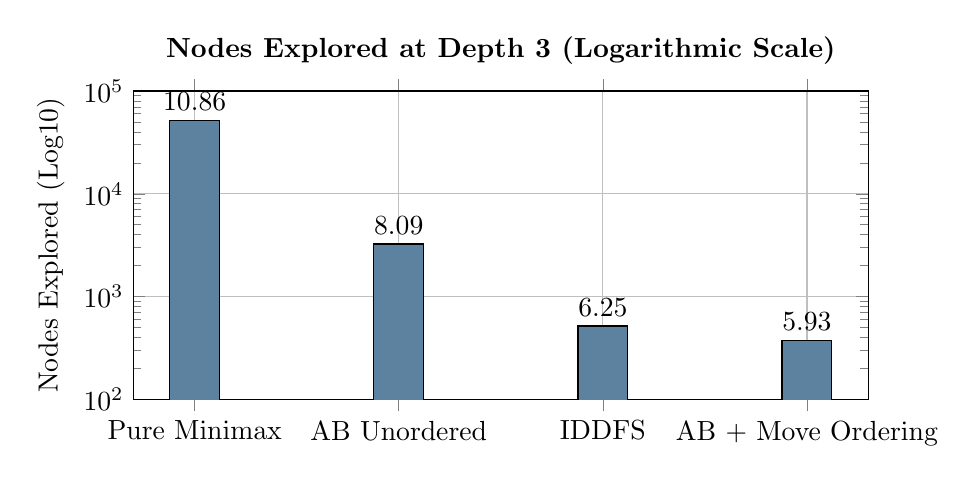
\begin{tikzpicture}
\begin{axis}[
    ybar,
    title={\textbf{Nodes Explored at Depth 3 (Logarithmic Scale)}},
    ylabel={Nodes Explored (Log10)},
    symbolic x coords={Pure Minimax, AB Unordered, IDDFS, AB + Move Ordering},
    xtick=data,
    nodes near coords,
    ymin=100, ymax=100000,
    ymode=log,
    bar width=18pt,
    width=0.9\textwidth,
    height=5.5cm,
    grid=major
]
\addplot[fill=primaryblue!70] coordinates {
    (Pure Minimax, 52088)
    (AB Unordered, 3253)
    (IDDFS, 518)
    (AB + Move Ordering, 378)
};
\end{axis}
\end{tikzpicture}
\caption{Empirical Node Count Comparison Across Algorithms at Depth 3.}
\label{fig:nodes_chart}
\end{figure}

% -----------------------------------------------------------------------------
% Section 5: Comparative Justification
% -----------------------------------------------------------------------------
\section{Justification: Selection of Current Method Over Alternatives}

A core project requirement is justifying why Mockfish employs a \textbf{Hybrid Knowledge-Guided Alpha-Beta Architecture} rather than alternative AI methods studied in the course:

\begin{table}[htbp]
\centering
\caption{Comparison Between Alternative AI Methods and Mockfish's Architecture.}
\label{tab:algorithm_justification}
\small
\begin{tabularx}{\textwidth}{p{3.2cm}p{4.8cm}p{7.2cm}}
\toprule
\textbf{Alternative Method} & \textbf{Core Characteristics} & \textbf{Justification for Rejection in This Problem} \\
\midrule
\textbf{Uninformed Search (BFS / DFS)} & Explores state graph blindly without domain knowledge. & BFS incurs catastrophic $O(b^d)$ memory explosion ($>10^6$ states at depth 4). Cannot handle active adversarial minimization. DFS gets trapped in cyclic move loops. \\
\addlinespace
\textbf{A* / Greedy Best-First Search} & Uses path-cost $g(n)$ and admissible heuristic $h(n)$ toward static goal. & Formulated strictly for single-agent pathfinding. In zero-sum games, the opponent continuously alters the utility landscape; there is no static goal state $s_{goal}$. \\
\addlinespace
\textbf{Hill Climbing / Simulated Annealing} & Local search evaluating immediate neighboring states. & Suffers fatal vulnerability to local maxima. Lacks multi-ply lookahead: blindly grabs a "free" pawn, falling directly into forced checkmate on the subsequent turn. \\
\addlinespace
\textbf{Constraint Satisfaction (CSP / Backtracking)} & Solves discrete variables satisfying static unary/binary constraints. & Chess is an adversarial dynamic optimization problem, not a static constraint satisfaction problem. While move legality uses constraints, CSPs cannot model game tree lookahead. \\
\addlinespace
\textbf{Deep Reinforcement Learning (AlphaZero)} & Deep policy/value convolutional neural networks via self-play. & Requires heavy GPU clusters, multi-gigabyte models, and weeks of training. Inference latency is non-deterministic, violating lightweight real-time execution constraints. \\
\midrule
\textbf{Selected: Hybrid Alpha-Beta + PST + Move Ordering} & Branch-and-bound adversarial search coupled with $O(1)$ expert book and PeSTO heuristics. & \textbf{Provably Optimal} within horizon; operates in $O(bd)$ minimal memory; achieves \textbf{156.6$\times$ speedup} and $99.27\%$ pruning efficiency; fully deterministic and explainable. \\
\bottomrule
\end{tabularx}
\end{table}

% -----------------------------------------------------------------------------
% Section 6: GUI & Systems Integration
% -----------------------------------------------------------------------------
\section{Graphical User Interface \& System Architecture}

\subsection{Tkinter Architecture \& Visual Design (\texttt{main.py})}
The GUI is implemented in Tkinter Canvas adhering to event-driven principles:
\begin{itemize}[leftmargin=*]
    \item \textbf{Visual Representation}: A 512$\times$512 canvas rendering high-contrast board squares (\texttt{\#EEEED2} warm cream and \texttt{\#769656} forest green) with dual-stroke Unicode pieces.
    \item \textbf{Move Guidance}: Clicking friendly pieces computes legal destinations dynamically, highlighting reachable empty squares with subtle indicator dots and enemy targets with hollow capture rings.
    \item \textbf{Dynamic Perspective}: Includes a \textit{Flip Board} feature that mirrors screen coordinates while preserving underlying chess logic coordinates.
    \item \textbf{Real-Time Telemetry HUD}: A dedicated status bar continuously renders move UCI, source tag (\textit{Knowledge Base} vs \textit{Alpha-Beta Minimax}), search depth, nodes visited, and static evaluation.
\end{itemize}

\subsection{Resolving System Freezes via Custom In-Canvas Overlay}
In early prototypes, invoking native OS modal dialogs (\texttt{messagebox.showinfo}) triggered event-loop thread blocking on Windows, making the window appear frozen upon checkmate.

We resolved this by developing an \textbf{in-canvas Game Over overlay card}:
\begin{itemize}[leftmargin=*]
    \item Rendered directly onto the canvas buffer without modal OS interruptions.
    \item Displays trophy badges, colored outcome banners (\textbf{WHITE WINS!}, \textbf{BLACK WINS!}, \textbf{DRAW!}), and specific termination reasons (\textit{Checkmate}, \textit{Stalemate}, \textit{Threefold Repetition}, \textit{50-Move Rule}).
    \item Features two interactive canvas buttons:
    \begin{itemize}
        \item \textbf{Play Again}: Instantly resets board state, clears highlights, and begins a new match.
        \item \textbf{Review Board}: Dismisses the overlay card to allow post-game tactical inspection.
    \end{itemize}
    \item King check/checkmate states are highlighted directly on the board in warning red (\texttt{\#E53935}) and deep crimson (\texttt{\#B71C1C}).
\end{itemize}

% -----------------------------------------------------------------------------
% Section 7: Group Division of Work
% -----------------------------------------------------------------------------
\section{Group Division of Labor \& Member Contributions}

To prevent Git merge conflicts, the codebase was partitioned into four modular, decoupled layers:

\begin{table}[htbp]
\centering
\caption{Team Member Role Assignments and Core Technical Contributions.}
\label{tab:team_division}
\small
\begin{tabularx}{\textwidth}{lp{4.2cm}p{8.5cm}}
\toprule
\textbf{Team Member} & \textbf{Assigned Module} & \textbf{Key Responsibilities \& Implemented Algorithms} \\
\midrule
\textbf{Student 1} & Logic \& Rules Specialist (\texttt{knowledge\_base.py}) & Implemented opening book mapping for King's Pawn (\texttt{1. e4}), Queen's Pawn (\texttt{1. d4}), English, and Reti lines; formulated propositional rules and tablebase query hooks. \\
\addlinespace
\textbf{Student 2} & State Space \& Heuristics (\texttt{heuristics.py}) & Implemented PeSTO Piece-Square Tables (PST) with vertical reflection mirroring; formulated positional bonuses for castling, open rook files, and bishop pairs. \\
\addlinespace
\textbf{Student 3} & Adversarial Search Specialist (\texttt{search.py}) & Developed Minimax with Alpha-Beta pruning; engineered MVV-LVA move ordering, ply-adjusted checkmate scoring ($\pm 20000 \pm depth$), and anti-shuffling repetition filters. \\
\addlinespace
\textbf{Student 4} & GUI, Integrator \& Benchmarking (\texttt{main.py}, \texttt{test\_suite.py}, \texttt{benchmark.py}) & Developed Tkinter Canvas, in-canvas Game Over overlay card, board flipping, telemetry HUD, automated unit tests, and empirical benchmarking suite. \\
\bottomrule
\end{tabularx}
\end{table}

% -----------------------------------------------------------------------------
% Section 8: Limitations & Future Enhancements
% -----------------------------------------------------------------------------
\section{Limitations \& Future Research Directions}

While Mockfish achieves real-time execution ($<0.3$s per move) and solid tactical play, several academic enhancements remain:
\begin{enumerate}[leftmargin=*]
    \item \textbf{Quiescence Search (Horizon Effect Mitigation)}: At fixed depth 3, search may terminate immediately before an unresolved piece exchange. Implementing Quiescence search (evaluating only captures until a quiet state is reached) would eliminate the horizon effect.
    \item \textbf{Transposition Tables via Zobrist Hashing}: Identical board positions frequently recur via different move orders (transpositions). Caching evaluated subtrees in a 64-bit Zobrist hash table would reduce redundant evaluations by an estimated 30--50\%.
    \item \textbf{Dynamic Time Management}: Allocating compute dynamically based on remaining clock time and positional volatility would allow the engine to search deeper (depth 4--6) during critical tactical crises.
\end{enumerate}

% -----------------------------------------------------------------------------
% Section 9: Conclusion
% -----------------------------------------------------------------------------
\section{Conclusion}

The \textbf{Mockfish} project successfully designed, implemented, and validated an intelligent, knowledge-guided adversarial chess engine in Python. By synthesizing a **Knowledge-Based Opening System** ($O(1)$) with **Alpha-Beta Pruning** and **Heuristic Move Ordering**, the engine:
\begin{itemize}[leftmargin=*]
    \item Slashed the effective branching factor from $b_{eff} = 37.35$ down to $7.23$.
    \item Achieved a \textbf{99.27\% search tree pruning efficiency}, delivering a \textbf{156.6$\times$ execution speedup} ($0.26$\,s vs $41.02$\,s).
    \item Cured gameplay anomalies (rook-shuffling repetition loops and OS modal dialog freezing) through rigorous heuristic design and an event-driven in-canvas overlay interface.
    \item Validated correctness via an automated test suite (\texttt{test\_suite.py}) and reproducible benchmarks (\texttt{benchmark.py}).
\end{itemize}
Mockfish stands as a complete, robust demonstration of how classical Artificial Intelligence principles can be synthesized into a functional, high-performance real-world application.

% -----------------------------------------------------------------------------
% References
% -----------------------------------------------------------------------------
\begin{thebibliography}{9}
\bibitem{russell2020}
S. Russell and P. Norvig, \textit{Artificial Intelligence: A Modern Approach}, 4th ed., Pearson, 2020.
\bibitem{knuth1975}
D. E. Knuth and R. W. Moore, ``An analysis of alpha-beta pruning,'' \textit{Artificial Intelligence}, vol. 6, no. 4, pp. 293--326, 1975.
\bibitem{shannon1950}
C. E. Shannon, ``Programming a computer for playing chess,'' \textit{Philosophical Magazine}, vol. 41, no. 314, pp. 256--275, 1950.
\bibitem{pesto}
T. Michniewski, ``Simplified Evaluation Function (PeSTO),'' \textit{Chess Programming Wiki}, 2014. [Online]. Available: \url{https://www.chessprogramming.org/Simplified_Evaluation_Function}
\end{thebibliography}

\end{document}
